
\documentclass[paper=a4, fontsize=11pt]{scrartcl} % A4 paper and 11pt font size


\usepackage{graphicx}
\graphicspath{ {images/} }
\usepackage{bm}
\usepackage[T1]{fontenc} % Use 8-bit encoding that has 256 glyphs
\usepackage{fourier} % Use the Adobe Utopia font for the document - comment this line to return to the LaTeX default
\usepackage[english]{babel} % English language/hyphenation
\usepackage{amsmath,amsfonts,amsthm} % Math packages

\usepackage{sectsty} % Allows customizing section commands
%\allsectionsfont{\centering \normalfont\scshape} % Make all sections centered, the default font and small caps

\usepackage{datetime}
\usepackage{fancyhdr} % Custom headers and footers
\DeclareMathOperator*{\argmax}{argmax}
\newcommand*{\argmaxl}{\argmax\limits}
\pagestyle{fancyplain} % Makes all pages in the document conform to the custom headers and footers
\fancyhead{} % No page header - if you want one, create it in the same way as the footers below
\fancyfoot[L]{} % Empty left footer
\fancyfoot[C]{} % Empty center footer
\fancyfoot[R]{\thepage} % Page numbering for right footer
\renewcommand{\headrulewidth}{0pt} % Remove header underlines
\renewcommand{\footrulewidth}{0pt} % Remove footer underlines
\setlength{\headheight}{13.6pt} % Customize the height of the header

\numberwithin{equation}{section} % Number equations within sections (i.e. 1.1, 1.2, 2.1, 2.2 instead of 1, 2, 3, 4)
\numberwithin{figure}{section} % Number figures within sections (i.e. 1.1, 1.2, 2.1, 2.2 instead of 1, 2, 3, 4)
\numberwithin{table}{section} % Number tables within sections (i.e. 1.1, 1.2, 2.1, 2.2 instead of 1, 2, 3, 4)

\setlength\parindent{0pt} % Removes all indentation from paragraphs - comment this line for an assignment with lots of text

%----------------------------------------------------------------------------------------
%	TITLE SECTION
%----------------------------------------------------------------------------------------

\newcommand{\horrule}[1]{\rule{\linewidth}{#1}} % Create horizontal rule command with 1 argument of height

\title{	
\normalfont \normalsize 
\textsc{Indraprastha Institute of Information Technology, Delhi} \\ [25pt] % Your university, school and/or department name(s)
\horrule{0.5pt} \\[0.4cm] % Thin top horizontal rule
\huge CSE561-Probabilistic Graphical Models : Project\\ % The assignment title
\horrule{2pt} \\[0.5cm] % Thick bottom horizontal rule
}

\author{Ashutosh Gupta and Sagar Verma} % Your name

\newdate{date}{26}{03}{2016}
\date{\normalsize\displaydate{date}} % Today's date or a custom date

\begin{document}

\maketitle % Print the title

%----------------------------------------------------------------------------------------
%	PROBLEM 1
%----------------------------------------------------------------------------------------

\section{Problem Description}

\subsection{Optical Word Recognition}

\par
Optical word recognition problem is the identification of word from a given image of characters. OWR is an extension of Optical character recognition. Through various comptuer vision techniques individual characters can be obtained from an image with certain probability for each characer for a single image. To construct meaningful word from those characters we need prior probablities of occurence of one character after another. This whole problem can be represented as a graphical model and maximum probable explanation(MAP) of the model gives the probable word the image is showing. 

\par
In given problem we have $1000$ image ids and for each image id we have $10$ characters and their factors. This factors represent the certainity with which each character is the content of that image. Transition factors between every two characters is given. Skip factor is given if two same image ids means same characters which is $5.0$ otherwise $1.0$. Given these factors, the probability to the character variables of a word $w$ according to model will be given by:


\begin{align*}
			p(chars) = \dfrac{1}{z} \begin{pmatrix}
										 \displaystyle \prod_{\forall i}^{} & \psi_{o}\big(img(i),char(i)\big) \\
										 \displaystyle \prod_{i=0,...,|w|-2}^{} & \psi_{t}\big(char(i),char(i+1)\big) \\
										 \displaystyle \prod_{i,j|img(i)=img(j)}^{} & \psi_{s}\big(char(i),char(i)\big) \\
									\end{pmatrix}
\end{align*}

where $\psi_o$ is OCR factor, $\psi_t$ is transition factor and $\psi_s$ is skip factor.

\section{Solution Approach}

\subsection{Undirected Graphical Model}
Assume a word consisting $n$ characters and it formed of $n$ images. Graphically this can be represented as below

\begin{figure}[!ht]
	\centering
		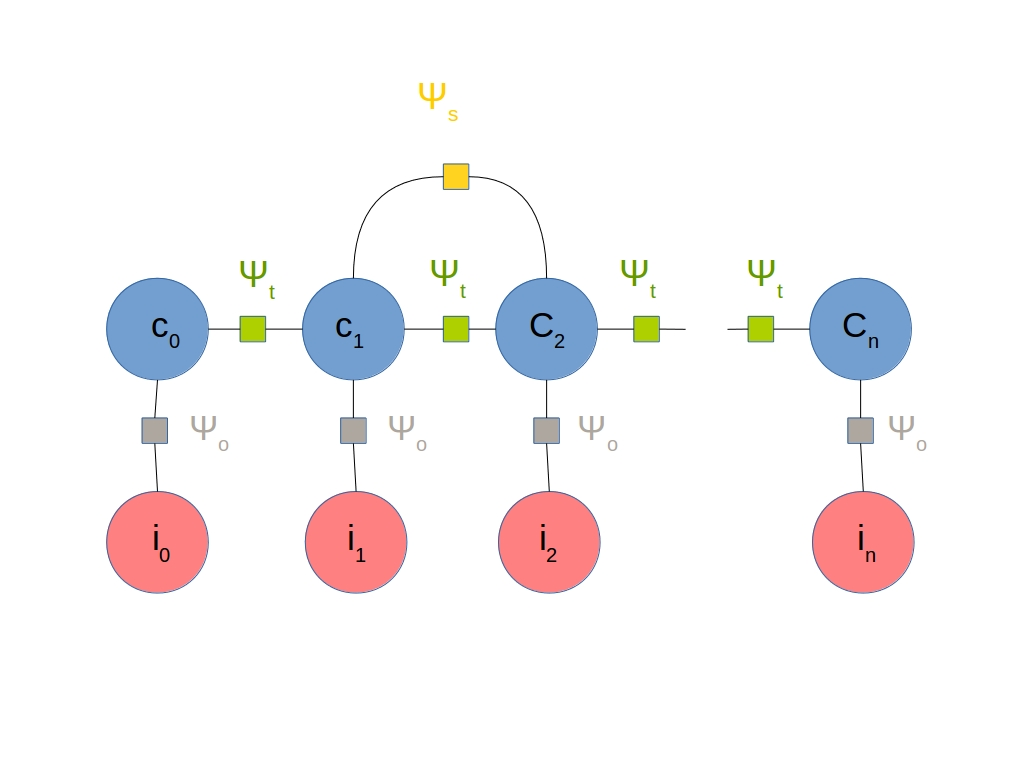
\includegraphics[scale=0.4]{model}
		\caption{OWR problem as Undirected Graphical Model}
\end{figure}

\subsubsection{OCR Model}

\par
OCR model contains only OCR factors i.e. $\psi_o$. Most probable explanation can be calculated as,

\begin{align*}
	\tilde{p}(chars) & = \argmaxl_{c_0,c_1,...c_n} \tilde{p}(c_0,c_1,...c_n) \\
					 & = \argmaxl_{c_0,c_1,...c_n} \bigg(\displaystyle \prod_{\forall i}^{}  \psi_{o}\big(img(i),char(i)\big) \bigg)\\
\end{align*}

Partition function, $z$ can be calculated as,

\begin{align*}
	z & = \displaystyle \sum_{\psi_{o}}^{} \bigg(\displaystyle \prod_{\forall i}^{}  \psi_{o}\big(img(i),char(i)\big) \bigg)\\
\end{align*}

Pobability of word can be calculated as,

\begin{align*}
	p(chars) = \dfrac{1}{z} \tilde{p}(chars) \\
\end{align*}

\subsection{Transition Model}



\par
Transition model contains both OCR factors and transition factors. Most probable explanation can be calculated as,

\begin{align*}
	\tilde{p}(chars) & = \argmaxl_{c_0,c_1,...c_n} \tilde{p}(c_0,c_1,...c_n,i_0,i_1,...,i_n) \\
					 & = \argmaxl_{c_0,c_1,...c_n} \bigg( \displaystyle \prod_{\forall i}^{}  \psi_{o}\big(img(i),char(i)\big) \displaystyle \prod_{i=0,...,|w|-2}^{}  \psi_{t}\big(char(i),char(i+1)\big) \bigg)\\
\end{align*}

Partition function, $z$ can be calculated as,

\begin{align*}
	z & = \displaystyle \sum_{\psi_{o} \psi_{t}}^{} \bigg( \displaystyle \prod_{\forall i}^{}  \psi_{o}\big(img(i),char(i)\big) \displaystyle \prod_{i=0,...,|w|-2}^{}  \psi_{t}\big(char(i),char(i+1)\big) \bigg)\\
\end{align*}

Pobability of word can be calculated as,

\begin{align*}
	p(chars) = \dfrac{1}{z} \tilde{p}(chars) \\
\end{align*}

\subsection{Combined Model}

Combined model contains OCR factors, transition factors and Skip factors. Most probable explanation can be calculated as,

\begin{align*}
	\tilde{p}(chars) & = \argmaxl_{c_0,c_1,...c_n} \tilde{p}(c_0,c_1,...c_n,i_0,i_1,...,i_n) \\
					 & = \argmaxl_{c_0,c_1,...c_n} \bigg( \displaystyle \prod_{\forall i}^{}  \psi_{o}\big(img(i),char(i)\big) \displaystyle \prod_{i=0,...,|w|-2}^{}  \psi_{t}\big(char(i),char(i+1)\big) \\ & \displaystyle \prod_{i,j|img(i)=img(j)}^{} \psi_{s}\big(char(i),char(i)\big) \bigg)\\
\end{align*}

Partition function, $z$ can be calculated as,

\begin{align*}
	z & = \displaystyle \sum_{\psi_{o} \psi_{t} \psi_{s}}^{} \bigg( \displaystyle \prod_{\forall i}^{}  \psi_{o}\big(img(i),char(i)\big) \displaystyle \prod_{i=0,...,|w|-2}^{}  \psi_{t}\big(char(i),char(i+1)\big) \\ & \displaystyle \prod_{i,j|img(i)=img(j)}^{} \psi_{s}\big(char(i),char(i)\big) \bigg)\\
\end{align*}

Pobability of word can be calculated as,

\begin{align*}
	p(chars) = \dfrac{1}{z} \tilde{p}(chars) \\
\end{align*}

\section{Results Obtained}

Exhaustive inference can be done by calculating probabilities for all possible words for given set of images. To find most probable explanation(MPE) or MAP, juntion tree algorithm is used. Python has a pyMNS library which has JTA implimentation \cite{pymns}.

\begin{table}[h!]
  \begin{center}
    \begin{tabular}{||c c c c||} 
    \hline
      Model & Char Accuracy & Word Accuracy & Log Likelihood \\ [0.5ex] 
    \hline\hline
      OCR &  0.53921 & 0.08653 & -7.54175 \\ 
    \hline
      Transition & 0.66274 & 0.259615 & -6.88575 \\
    \hline
      Combined &  0.71176 & 0.355769 & -6.102387 \\
    \hline
    \end{tabular}
    \caption{Model Accuracy} \label{table:1}
  \end{center}
\end{table}

Table \ref{table:1} shows character-wise accuracy, word-wise accuracy and average dataset log-likelihood for all three models. From the results we can see that combined model performs best out of the three models and OCR model performs the worst.


\section{Further Fun}

\par

Varying the potentials has no effect on the word predicted or the accuracy calulated. Exhaustive inference for OCR model can be calulated using matrix multiplication which is faster than generating all possible words and calculating probabilites for each of them.

\subsection{Directed Model}

\begin{figure}[!ht]
	\centering
		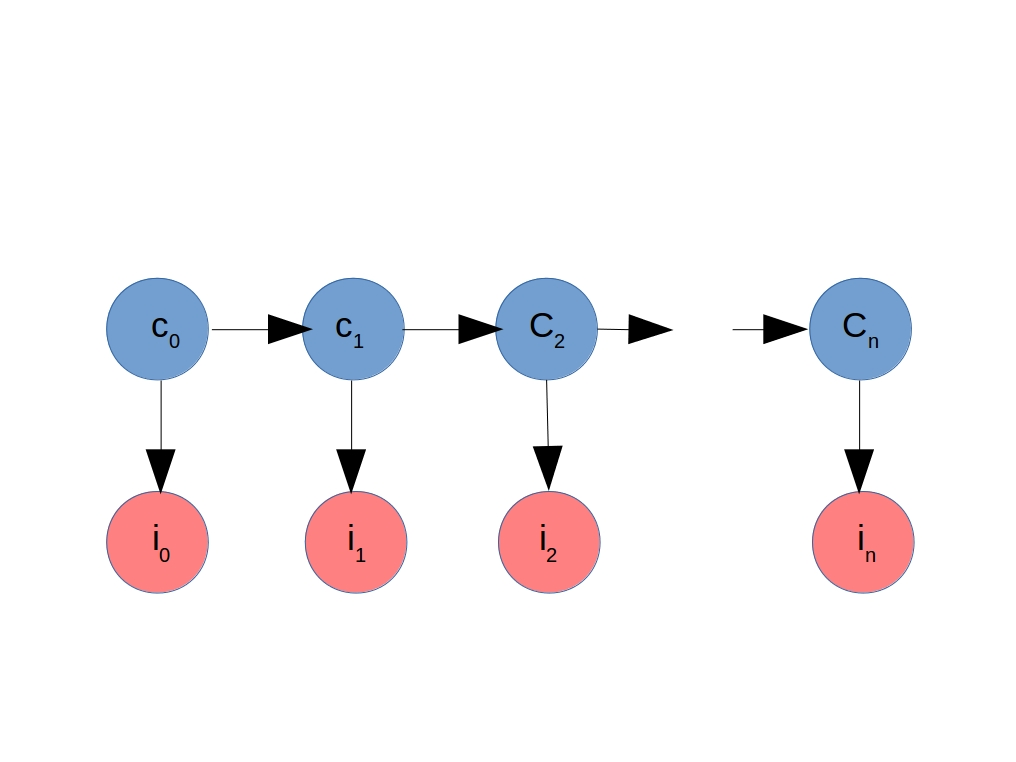
\includegraphics[scale=0.4]{bnet}
		\caption{Directed Graphical Model}
\end{figure}

MAP can be calculated as,
\begin{align*}
	\argmaxl_{c_0,c_1,...,c_n} P(c_0,c_1,..c_n,i_0=I_0,i_1=I_1,...,i_n=I_n) = &\argmaxl_{c_0,c_1,...,c_n} \Big( p(c_0)p(c_1c_0)...p(c_n|c_{n-1})p(i_0=I_0|c_0) \\
	 																			&p(i_1=I_1|c_1)...p(i_n=I_n|c_n)\Big) \\
\end{align*}

MAP for bayesian network is found using libpgm python library \cite{libpgm}.

\section{Appendix}

\begin{itemize}
  \item \textit{all\_code.py} does exhaustive reference, finds model accuracy and print outcomes.
  \item \textit{basian\_creator.py} creates JSON file representing bayesian networks.
  \item \textit{bayesian\_solver.py} solves bayesian network and gives probability of finding true word given image ids as evidence.
  \item \textit{parallel\_code.py} is faster implimentation of OCR model using matrix multiplication.
  \item \textit{furthe\_fun.py} uses pyMNS to solve markov net using JTA \cite{pymns}.
  \item \textit{bayes\_net} contains all JSON files of bayesian networks.
  \item \textit{dataset} contains datasets.
  \item \textit{docs} contains report files.
  \item \textit{probs} contains markov net files.
\end{itemize}


\begin{thebibliography}{9}
\bibitem{pymns}
Python Markov network solver library,
\texttt{https://github.com/daveti/pymns}

\bibitem{libpgm}
Python Bayesian network solver library,
\texttt{http://pythonhosted.org/libpgm/}

\end{thebibliography}
\end{document}